\chapter{Implementation of Gradient Boosting}
\label{ch:gbm}

%=============================================================================
\section{Pipeline overview}
\label{sec:lgbm-pipeline}
%=============================================================================

Gradient boosting is implemented as the first of the two machine-learning
baselines compared against Ordinary Kriging in
Chapter~\ref{ch:comparison}. The model is a direct probabilistic
regressor: the additive ensemble of Equation~\eqref{eq:gbm-additive} is
trained independently for a discrete grid of quantile levels using the
pinball loss of Equation~\eqref{eq:pinball}, so each station-day receives
an empirical predictive distribution rather than a single point
estimate. Three properties make LightGBM
\cite{ke2017lightgbm} a practical fit for this dataset: histogram-based
splitting (Section~\ref{sec:theory-lgbm}) handles the 17.4-million
wet-day records of the 1961--2023 archive without exhausting memory;
auxiliary covariates such as elevation and soil properties enter the
model directly, with no parametric stationarity assumption; and the
pinball objective is supported as a built-in loss, so the eleven
quantile boosters jointly form the predictive ensemble required for
CRPS evaluation (Section~\ref{sec:theory-crps}).

The same two-stage decomposition $Z = I \cdot A$ used by
Ordinary Kriging (Section~\ref{sec:kriging-indicator}) is preserved.
\emph{Stage~1} is a binary \texttt{LGBMClassifier} predicting the
wet-day indicator, which replaces indicator kriging and uses the
$\hat{p} > 0{.}4$ decision threshold of Hofstra et
al.~\cite{hofstra2008comparison}. \emph{Stage~2} is the eleven
quantile boosters trained on wet days only, which replace amount
kriging. The cells classified as dry by Stage~1 are clipped to zero
and bypass Stage~2. Figure~\ref{fig:lgbm-pipeline} illustrates the
full pipeline.

\begin{figure}[H]
    \centering
    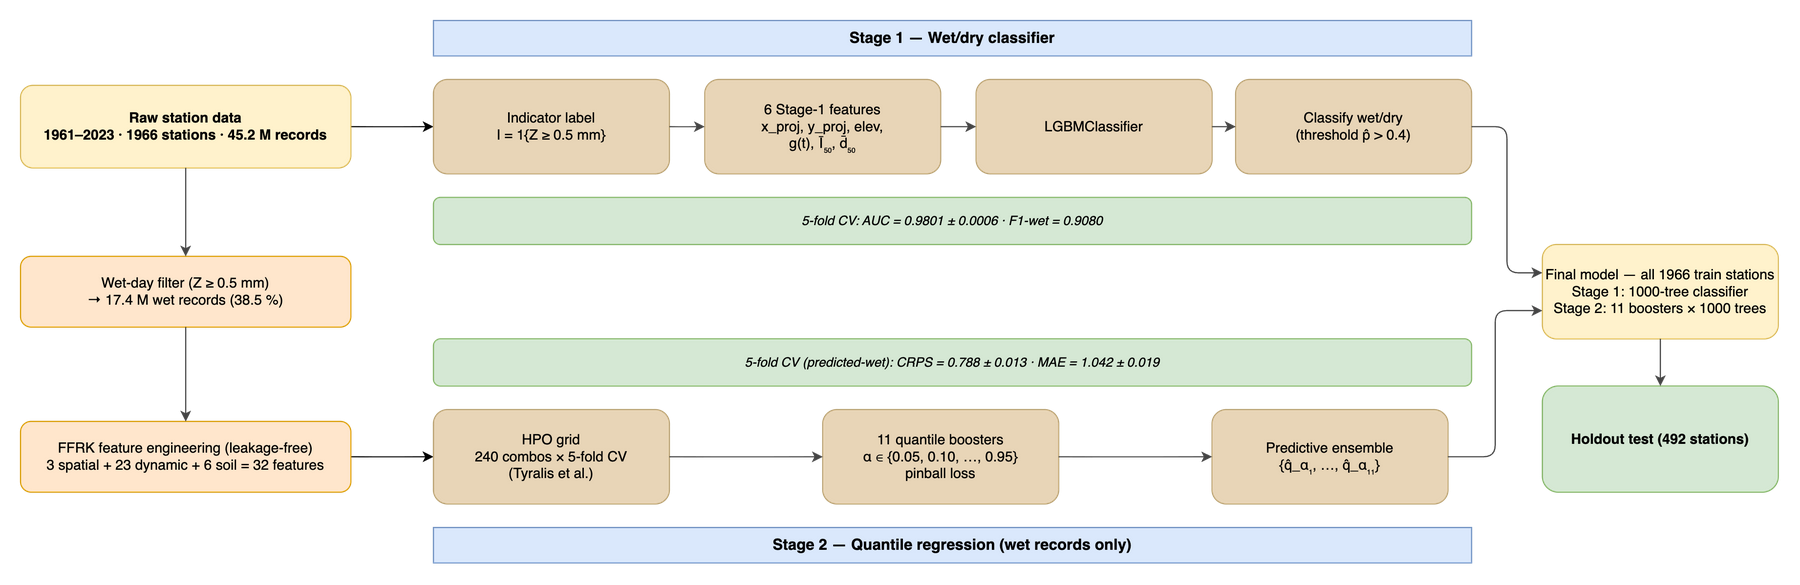
\includegraphics[width=\textwidth]{images/05/lgbm_pipeline}
    \caption{LightGBM two-stage pipeline. Stage~1 predicts the wet/dry
    indicator; Stage~2 trains eleven quantile boosters on wet records;
    HPO precedes Stage~2 training}
    \label{fig:lgbm-pipeline}
\end{figure}

%=============================================================================
\section{Stage~1: wet/dry classifier}
\label{sec:lgbm-stage1}
%=============================================================================

Stage~1 is a binary \texttt{LGBMClassifier} that predicts the wet-day
indicator $I(\mathbf{s}, t) = \mathbf{1}\{Z(\mathbf{s}, t) \ge
0{.}5\,\mathrm{mm}\}$ at every query location and date. Its feature
set is smaller than the 32-feature Stage~2 vector of
Section~\ref{sec:lgbm-features}: predicting whether it rained is a
binary decision dominated by the synoptic state and the local rainfall
area, whereas predicting \emph{how much} requires the full
distributional encoding of the neighbourhood. The six Stage~1 features
are listed in Table~\ref{tab:lgbm-stage1-features}.

\begin{table}[ht]
  \centering
  \caption{Input features for the LightGBM Stage~1 wet/dry classifier.
  The two kNN features pool the wet/dry indicator and the distance over
  the $K = 50$ nearest training neighbours of the query station; the
  global wet fraction is the per-day fraction of training stations with
  $Z \ge 0{.}5\,\mathrm{mm}$}
  \label{tab:lgbm-stage1-features}
  \begin{tabular}{l l l}
    \toprule
    Feature & Definition & Type \\
    \midrule
    $x_{\mathrm{proj}}$        & EPSG:3035 easting   & static  \\
    $y_{\mathrm{proj}}$        & EPSG:3035 northing  & static  \\
    \texttt{elevation\_m}      & Copernicus DEM-30   & static  \\
    \texttt{global\_wet\_frac} &
      $g(t) = \frac{1}{|\mathcal{S}_{\mathrm{tr}}|}
        \sum_{\mathbf{s} \in \mathcal{S}_{\mathrm{tr}}} I(\mathbf{s}, t)$
                                                    & per day \\
    \texttt{knn\_wet\_frac}    &
      $\bar{I}_K(\mathbf{s}, t) =
        \frac{1}{K} \sum_{j \in \mathcal{N}_K(\mathbf{s})} I(j, t)$
                                                    & per day \\
    \texttt{knn\_mean\_dist\_km} &
      $\bar{d}_K(\mathbf{s}) =
        \frac{1}{K} \sum_{j \in \mathcal{N}_K(\mathbf{s})}
          \|\mathbf{s} - j\|$                       & static  \\
    \bottomrule
  \end{tabular}
\end{table}

The features encode two complementary spatial scales of evidence. The
global wet fraction $g(t)$ summarises the synoptic state of day $t$: a
frontal passage produces high $g$ across the entire domain, while a
fair-weather day produces low $g$ everywhere. The kNN wet fraction
$\bar{I}_K(\mathbf{s}, t)$ summarises the local rainfall pattern in
the immediate neighbourhood of $\mathbf{s}$ on the same day,
distinguishing the wet sub-regions of an otherwise dry day (and vice
versa). The number of neighbours used in the kNN features is
$K = 50$, larger than the $K = 15$ used by Stage~2. The wet/dry
indicator carries less spatial noise than the amount field, so
averaging fifty indicators yields a stable rainfall-area estimate,
whereas averaging fifty amounts would blur the convective structure
that Stage~2 needs to resolve. As with the Stage~2 dynamic features,
the neighbour pool for $\bar{I}_K$ and the denominator of $g$ are
restricted to training stations only, so no leakage from holdout or
from the held-out fold during cross-validation can occur.

\paragraph{Hyperparameters.}
\begin{sloppypar}
The Stage~1 booster is fitted with the binary cross-entropy objective
and the settings $\texttt{n\_estimators} = 1000$,
$\texttt{learning\_rate} = 0{.}05$, $\texttt{num\_leaves} = 63$,
$\texttt{min\_child\_samples} = 50$, $\texttt{feature\_fraction} = 0{.}8$,
$\texttt{bagging\_fraction} = 0{.}8$ and $\texttt{bagging\_freq} = 1$.
Class imbalance is handled by setting
$\texttt{scale\_pos\_weight} = n_{\mathrm{dry}} / n_{\mathrm{wet}}$
computed on each fold's training set. Stage~1 hyperparameters were not
tuned on a grid: cross-validation AUC was already $0{.}98$ at the
defaults above, leaving little headroom for further tuning, so the
search budget was spent on the Stage~2 grid of
Section~\ref{sec:lgbm-training} instead.
\end{sloppypar}

\paragraph{Decision threshold.} At pipeline-inference time, a
station-day is forwarded to Stage~2 when
$\hat{p}_{\mathrm{wet}} > 0{.}40$, the same threshold used by the
indicator kriging step (Section~\ref{sec:kriging-indicator}, Hofstra
et al.~\cite{hofstra2008comparison}). Records below the threshold
receive a predictive distribution that is a point mass at zero,
equivalently an eleven-member ensemble of zeros at the Stage~2
quantile grid, so that the joint distribution feeding CRPS is
well-defined for every record. Lowering the threshold from the
conventional $0{.}50$ to $0{.}40$ trades a small increase in false
alarms for a substantial reduction in missed events, which is the
more expensive error class in CRPS terms: a missed wet day pays the
full observed amount, whereas a false alarm only pays the Stage~2
mean of the predicted ensemble.

\paragraph{Cross-validation performance.} Five-fold spatial
cross-validation on the canonical fold assignment of
Section~\ref{sec:lgbm-training} returns
ROC-AUC~$= 0{.}9801 \pm 0{.}0006$, Brier score
$= 0{.}0954 \pm 0{.}0009$, F1 on the wet class
$= 0{.}9080 \pm 0{.}0009$ and F1 on the dry class
$= 0{.}8908 \pm 0{.}0011$, all reported at the conventional
$\hat{p}_{\mathrm{wet}} > 0{.}50$ decision boundary. These scores
mirror the indicator-kriging skill of
Section~\ref{sec:kriging-indicator-impl}: the wet/dry binary is
highly separable at the 1~km daily aggregation, with the global wet
fraction $g(t)$ supplying the synoptic state and the kNN wet
fraction $\bar{I}_{50}(\mathbf{s}, t)$ resolving the local rainfall
area. The final classifier deployed in the combined pipeline is
trained on all $\sim$45.2 million station-days from the 1{,}966
training stations to 1{,}000 boosting rounds, with the kNN-derived
features recomputed once at full network density.

Figure~\ref{fig:lgbm-stage1-day} illustrates the Stage~1 wet/dry
mask on 15 July 2001, a summer convective day on which rainfall is
confined to the northern half of the domain. The classifier
reproduces the wet/dry boundary at the spatial resolution of the
1~km grid; residual misclassifications are concentrated along the
boundary itself, where the underlying probability
$\hat{p}_{\mathrm{wet}}$ transitions smoothly through the $0{.}40$
threshold.

\begin{figure}[ht]
    \centering
    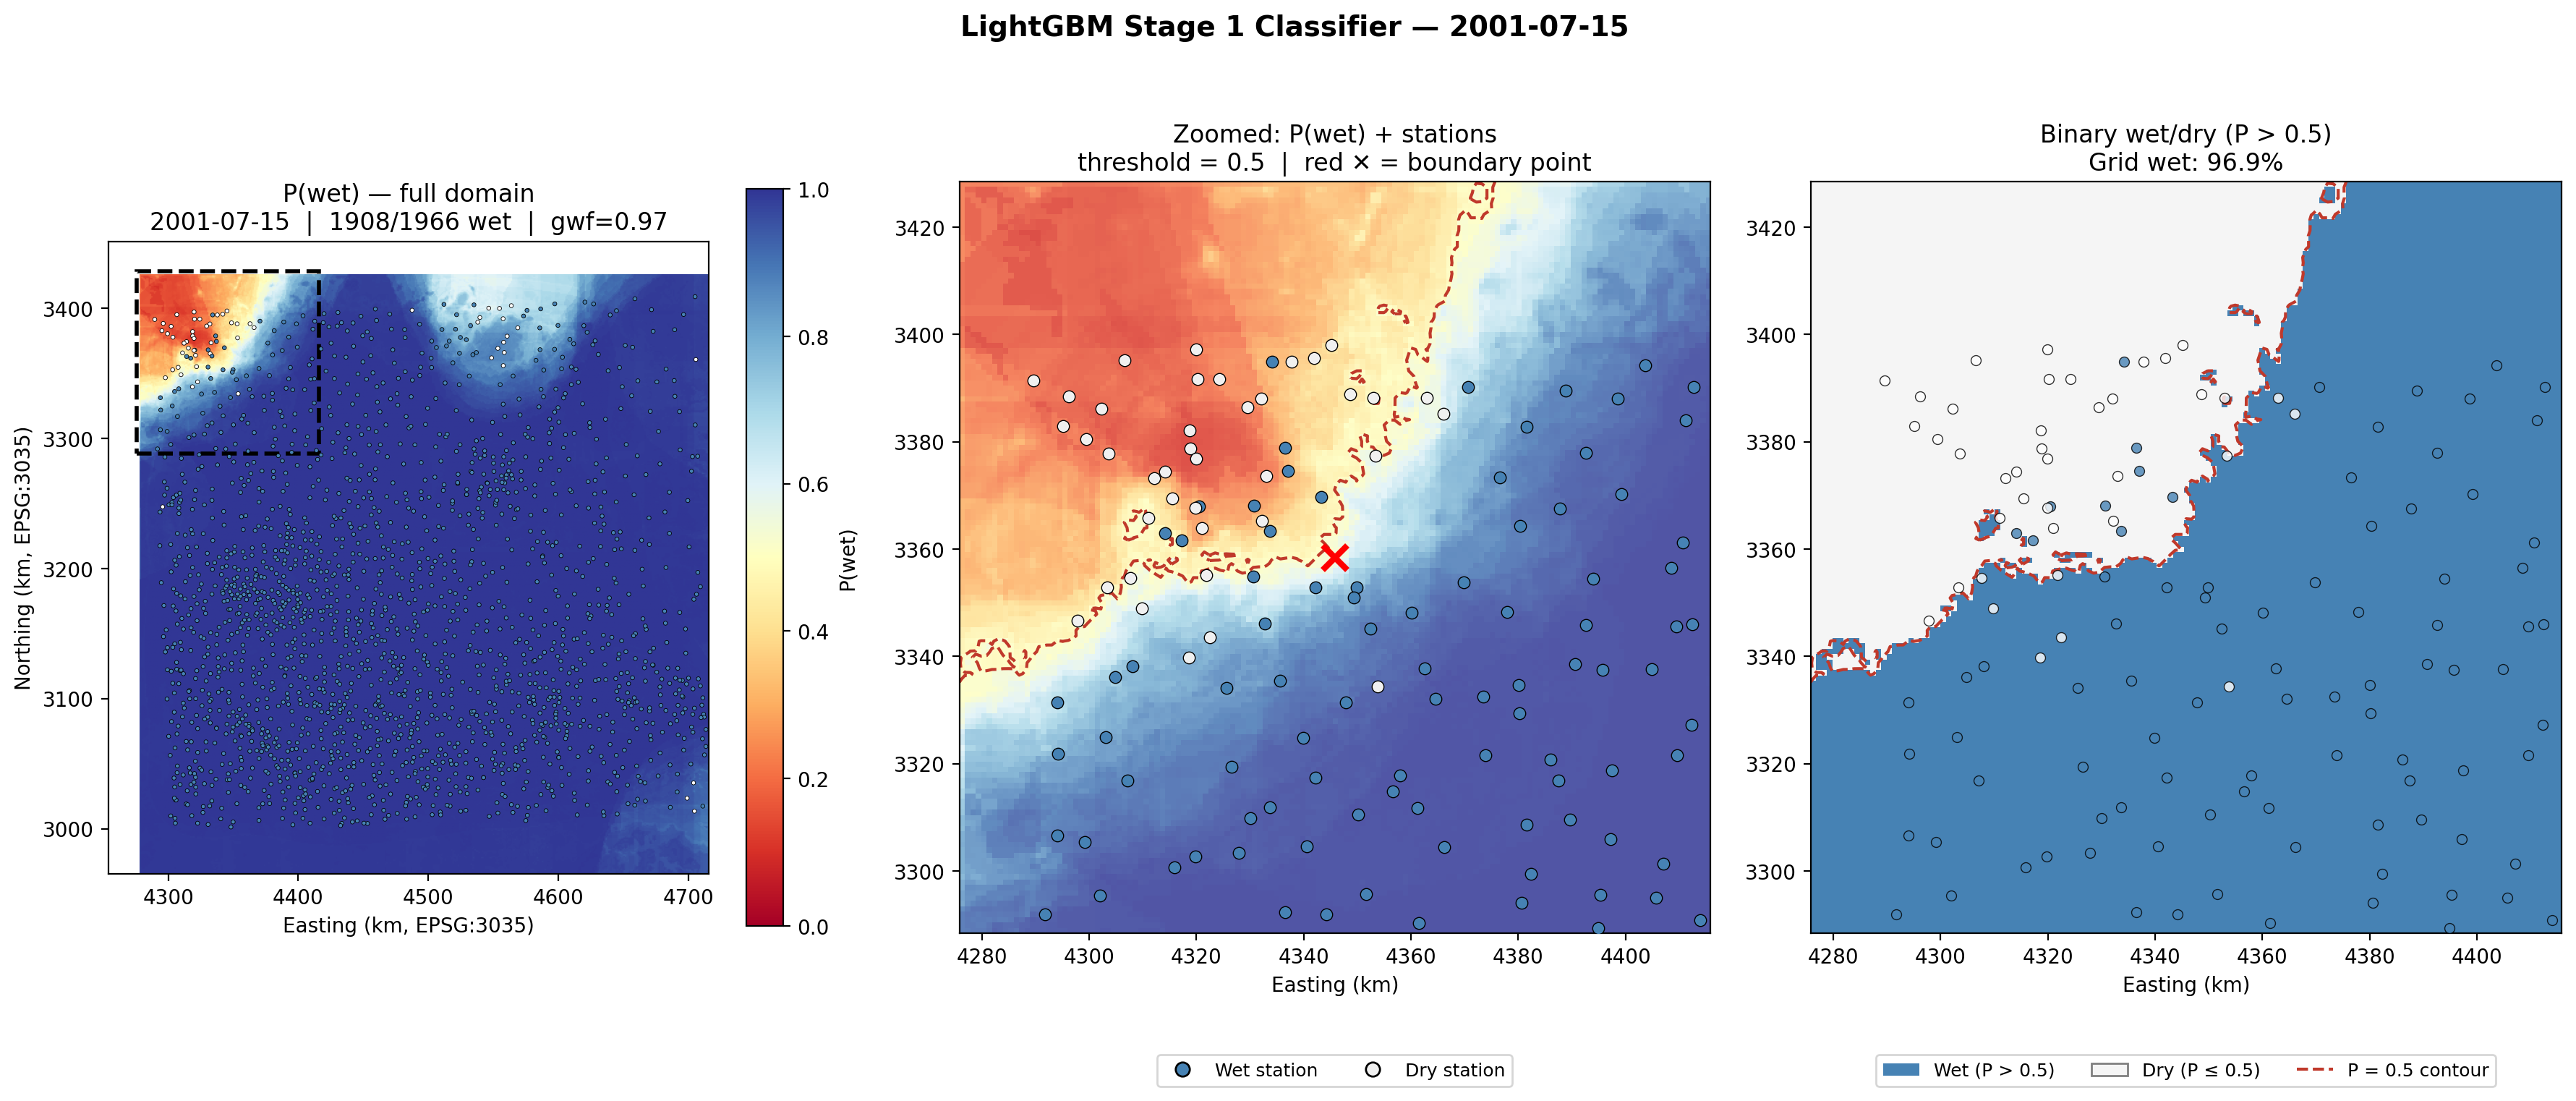
\includegraphics[width=0.95\textwidth]{images/05/lgbm_stage1_2001-07-15}
    \caption[Stage~1 wet/dry prediction for 15 July 2001]{Stage~1
    wet/dry prediction for 15 July 2001 on the 1~km EPSG:3035 grid.
    Left: predicted probability of rainfall $\hat{p}_{\mathrm{wet}}$.
    Right: binary wet/dry mask after applying the
    $\hat{p}_{\mathrm{wet}} > 0{.}40$ decision threshold. Station
    observations are overlaid as coloured discs}
    \label{fig:lgbm-stage1-day}
\end{figure}

%=============================================================================
\section{Stage~2: quantile regression}
\label{sec:lgbm-stage2}
%=============================================================================

\subsection{Why quantile regression}
\label{sec:lgbm-why-quantile}

Stage~2 predicts the rainfall amount conditional on a wet day. The
quantity of interest is not a single point estimate but the predictive
distribution $F_Z(z \mid \mathbf{s}, t)$, since CRPS
(Equation~\eqref{eq:crps}) and the calibration of prediction intervals
both require access to the full CDF. Quantile regression is the
natural fit for this requirement: a separate booster is trained for
each level $\alpha$ using the pinball loss
(Equation~\eqref{eq:pinball}), and the eleven predictions
$\{\hat{q}_{\alpha_1}, \ldots, \hat{q}_{\alpha_{11}}\}$ jointly form
an empirical predictive distribution that consumes the CRPS integrand
directly, with no parametric back-transformation. The two
alternatives explored before settling on direct quantile regression
were a regression-kriging hybrid (LightGBM trend plus Ordinary
Kriging on residuals) and parametric distribution-specific losses
(Tweedie, Gamma). The reasons for adopting direct quantile regression
are revisited in Section~\ref{sec:lgbm-discussion}.

\subsection{Feature engineering}
\label{sec:lgbm-features}

Gradient boosting requires that all spatial information be exposed as
explicit numerical features at the input layer. Whereas kriging
derives its spatial structure from the variogram, a tree ensemble has
no built-in notion of distance, isotropy or correlation: the network
geometry must be encoded manually. The feature engineering used here
follows the \emph{Feature-Free Regression Kriging} (FFRK) framework
of Luo, Wu and Song~\cite{luo2025featurefree}, in which three groups
of dynamic features (local dependence, local heterogeneity,
geosimilarity) capture the spatial structure that an external
covariate set would otherwise have to supply. To these dynamic
features, three projected spatial coordinates and six static
SoilGrids covariates are appended, yielding the 32-feature input
vector summarised in Table~\ref{tab:lgbm-features}.

\subsubsection*{Local dependence: inverse distance weighting}
\label{sec:lgbm-idw}

Local dependence is the tendency for nearby observations to take
similar values \cite{luo2025featurefree}. It is summarised at each
query location $\mathbf{s}_0$ by a single inverse-distance-weighted
average over its $K$ nearest wet-day neighbours
$\{\mathbf{s}_i\}_{i=1}^{K}$:
\begin{equation}
  f_{\mathrm{IDW}}(\mathbf{s}_0)
    = \frac{\sum_{i=1}^{K} w_i\, Z(\mathbf{s}_i)}{\sum_{i=1}^{K} w_i},
  \qquad
  w_i = \frac{1}{\|\mathbf{s}_0 - \mathbf{s}_i\|^{2} + \epsilon},
  \label{eq:lgbm-idw}
\end{equation}
with $K = 15$ and a numerical regulariser $\epsilon = 10^{-8}$~m$^2$
to prevent division by zero at coincident coordinates. The neighbour
count $K = 15$ is borrowed from the FFRK
paper~\cite{luo2025featurefree}, which adopts it from Song's GOS
work~\cite{song2022gos} and reports a sensitivity analysis confirming
the choice; the same value is therefore reused here without
re-tuning. The inverse-distance weighting produces a feature that
varies smoothly with the spatial density of nearby precipitation.
Because the same $K = 15$ neighbours are reused for the
heterogeneity and geosimilarity features below, the BallTree query
is performed once per day.

\subsubsection*{Local heterogeneity: SVD quantiles}
\label{sec:lgbm-svd}

A single weighted average compresses the neighbourhood into one
scalar and discards the shape of the local distribution. Local
heterogeneity is captured by encoding the empirical distribution of
the same $K$ neighbours as a vector of equally-spaced quantiles.
Following FFRK, twenty-one quantile levels
$\{0, 0{.}05, 0{.}10, \ldots, 0{.}95, 1\}$ are used:
\begin{equation}
  f_{\mathrm{SVD},q}(\mathbf{s}_0)
    = \mathrm{Quantile}_{q}\!\bigl(
        \{Z(\mathbf{s}_i)\}_{i=1}^{K}
      \bigr),
  \qquad q \in \{0, 0{.}05, \ldots, 1\},
  \label{eq:lgbm-svd}
\end{equation}
yielding twenty-one features \texttt{svd\_00}--\texttt{svd\_20}. The
full quantile profile encodes the minimum, median, maximum and
intermediate deciles of the local rainfall pattern in one shot,
exposing skewness and heavy-tail behaviour that an IDW average cannot
represent. The trees can then split on the upper-tail quantiles to
capture localised heavy events and on the lower-tail quantiles to
capture isolated dry patches inside a generally wet region.

\subsubsection*{Geosimilarity: GOS feature}
\label{sec:lgbm-gos}

Two query locations may share similar local rainfall
\emph{distributions} even when they are far apart, for instance two
stations in similar orographic settings on opposite sides of the
domain. The Geographically Optimal Similarity (GOS) framework of
Song~\cite{song2022gos} formalises this idea: the predictor at
$\mathbf{s}_0$ is a similarity-weighted mean of the values at
locations whose distributional profiles match that of $\mathbf{s}_0$.
Following FFRK, the profile vector at each neighbour is its own
SVD-quantile vector, the similarity is a Gaussian kernel of the
squared profile distance, and the GOS feature is the kernel-weighted
average:
\begin{equation}
  S_i =
    \exp\!\left(
      -\frac{
        \|\mathbf{p}_i - \mathbf{p}_0\|^{2}
      }{
        \sigma^{2}
      }
    \right),
  \qquad
  f_{\mathrm{GOS}}(\mathbf{s}_0)
    = \frac{\sum_{i=1}^{K} S_i\, Z(\mathbf{s}_i)}{\sum_{i=1}^{K} S_i},
  \label{eq:lgbm-gos}
\end{equation}
where $\mathbf{p}_0$ is the SVD-quantile vector at the query and
$\mathbf{p}_i$ at neighbour $i$, and $\sigma$ is a kernel bandwidth.
Compared with IDW, GOS down-weights neighbours whose distributional
shape diverges from the query's local pattern, even when they are
physically close, and up-weights neighbours that match the local
profile.

\subsubsection*{Static covariates}
\label{sec:lgbm-static}

The dynamic geo-features above describe the per-day point pattern but
encode no information about the underlying terrain or soil. Three
projected spatial coordinates and the six SoilGrids variables of
Section~\ref{sec:precip_statistics} are therefore appended as static
features: $x_{\mathrm{proj}}$ and $y_{\mathrm{proj}}$ in EPSG:3035
metres together with \texttt{elevation\_m} from the Copernicus DEM,
and the six SoilGrids predictors sampled at each station coordinate.

\subsubsection*{Feature inventory}
\label{sec:lgbm-feature-inventory}

Table~\ref{tab:lgbm-features} summarises the 32 input features that
enter each quantile booster. Three dynamic groups (IDW, SVD-quantiles,
GOS) are recomputed per day from the wet stations of that day; the
remaining nine features are station-level constants. The feature
importance ranking is reported in Section~\ref{sec:lgbm-discussion}.

\begin{table}[ht]
  \centering
  \caption{Input features for the LightGBM quantile boosters. The
  dynamic features (IDW, SVD, GOS) are recomputed each day from the
  $K = 15$ nearest wet-day neighbours; the static features are
  time-invariant per station}
  \label{tab:lgbm-features}
  \begin{tabular}{l c l l}
    \toprule
    Group              & Count & Source / formula
                                        & Type     \\
    \midrule
    Spatial            & 3     & EPSG:3035 + Copernicus DEM-30
                                        & static   \\
    IDW                & 1     & Equation~\eqref{eq:lgbm-idw}
                                        & per day  \\
    SVD-quantiles      & 21    & Equation~\eqref{eq:lgbm-svd}
                                        & per day  \\
    GOS                & 1     & Equation~\eqref{eq:lgbm-gos}
                                        & per day  \\
    SoilGrids          & 6     & SoilGrids 2.0 \cite{poggio2021soilgrids}
                                        & static   \\
    \midrule
    \textbf{Total}     & \textbf{32} &
                                        &          \\
    \bottomrule
  \end{tabular}
\end{table}

\subsection{Quantile grid and post-processing}
\label{sec:lgbm-quantiles}

The eleven quantile levels
\[
  \alpha \in
    \{0{.}05, 0{.}10, 0{.}20, 0{.}30, 0{.}40, 0{.}50,
      0{.}60, 0{.}70, 0{.}80, 0{.}90, 0{.}95\}
\]
are dense in the body of the distribution and span the central
90\,\% prediction interval at the extremes. One LightGBM booster is
trained independently for each $\alpha$ using the pinball loss of
Equation~\eqref{eq:pinball}; the ensemble of eleven predictions at
every station-day is the empirical predictive distribution that
feeds CRPS (Equation~\eqref{eq:crps}). Two cheap post-processing steps
are applied at inference time. First, each prediction is clipped to
be non-negative,
$\hat{q}_\alpha \leftarrow \max(\hat{q}_\alpha, 0)$, since
precipitation is non-negative. Second, the eleven predictions for a
given station-day are sorted in ascending order to repair occasional
quantile crossings introduced by the independent training of the
boosters. Both operations are deterministic and preserve the rank of
the predicted CDF.

\subsection{Training and hyperparameter tuning}
\label{sec:lgbm-training}

\paragraph{Data splitting.} The data partition follows
Section~\ref{sec:kriging-cv-methodology}: 1{,}966 train stations are
split into five folds via the canonical
\texttt{lgbm/fold\_assignment.parquet} file (${\sim}393$ stations
per fold), and the 492 holdout stations are reserved for the
cross-method evaluation of Chapter~\ref{ch:comparison}. The holdout
stations are excluded from hyperparameter optimisation, fold-level
training and feature recomputation, preventing leakage from train to
test through the dynamic geo-features.

\paragraph{Five-fold workflow.} Within each fold $k$, the four
other folds form the training set and the held-out fold is the test
set. Stage~1 is trained on every station-day record in the training
folds (wet and dry combined, $\sim$33~M records); Stage~2 is trained
only on the wet records ($\sim$13.9~M per fold). The dynamic
geo-features of Section~\ref{sec:lgbm-features} are recomputed for
every fold with the neighbour pool restricted to the four training
folds: a query station in the held-out fold $k$ retrieves its
$K = 15$ neighbours \emph{only from stations in folds $\ne k$}.
This prevents fold-internal information from leaking into the
test-fold features and is the LightGBM analogue of the fold-internal
variogram and monthly-normal refits used by Ordinary Kriging
(Section~\ref{sec:kriging-cv-methodology}).

\paragraph{Hyperparameter grid.}
\begin{sloppypar}
The four most influential LightGBM hyperparameters are tuned on a grid
inspired by Tyralis et al.~\cite{tyralis2023lightgbm}:
\texttt{max\_depth} $\in \{6, 8, 10\}$, \texttt{num\_leaves}
$\in \{20, 40, 60, 80, 100, 200, 500\}$ filtered to satisfy
$\texttt{num\_leaves} \le 2^{\texttt{max\_depth}}$,
\texttt{learning\_rate} $\in \{0{.}02, 0{.}05, 0{.}1\}$, and
\texttt{min\_child\_samples} $\in \{20, 100, 200, 500, 1000\}$.
After filtering, 240 valid combinations remain. Each combination is
evaluated by the mean CRPS across the five spatial folds defined
above. Per combination, the full quantile grid of
Section~\ref{sec:lgbm-quantiles} is trained on each fold, for a
total of $240 \times 11 \times 5 = 13{,}200$ boosters in the search.
\end{sloppypar}

\subsection{HPO results}
\label{sec:lgbm-hpo}

Figure~\ref{fig:lgbm-hpo} summarises the 240-combination grid
search. The left panel shows the marginal mean cross-validated CRPS
for each (\texttt{max\_depth}, \texttt{learning\_rate}) pair
averaged over leaves and minimum-child constraints; the three right
panels show the marginal distribution of cross-validated CRPS along
each remaining axis, with the within-axis minimum marked separately
from the within-axis mean. Cross-validated CRPS spans a narrow range
of $0{.}5195$--$0{.}5321$ across the grid (median $0{.}5231$,
standard deviation $0{.}003$), indicating that LightGBM is stable to
the choice of these four hyperparameters in the regime explored. This
narrow spread is partly attributable to the strong predictive signal of
the FFRK-derived geofeatures (Section~\ref{sec:lgbm-features}): IDW,
the SVD quantile profile and GOS already account for much of the
spatial and distributional structure, so the residual modelling task
faced by LightGBM is robust to hyperparameter perturbations within the
explored range. The
optimum lies at \texttt{max\_depth}~$= 10$,
\texttt{num\_leaves}~$= 200$, \texttt{learning\_rate}~$= 0{.}05$,
\texttt{min\_child\_samples}~$= 100$ with cross-validated mean
CRPS~$= 0.5195$~mm. Leaf-wise growth with a large leaf budget
benefits from the 13.9-million-record training pool, and the
$\texttt{min\_child\_samples}~= 100$ choice is a moderate
regularisation that prevents over-fitting on the dense central body
of the distribution while still letting the tail quantiles split.
This combination is fixed for the per-fold reporting of
Section~\ref{sec:lgbm-cv-results} and for the final all-data model
used in Chapter~\ref{ch:comparison}.

\begin{figure}[ht]
    \centering
    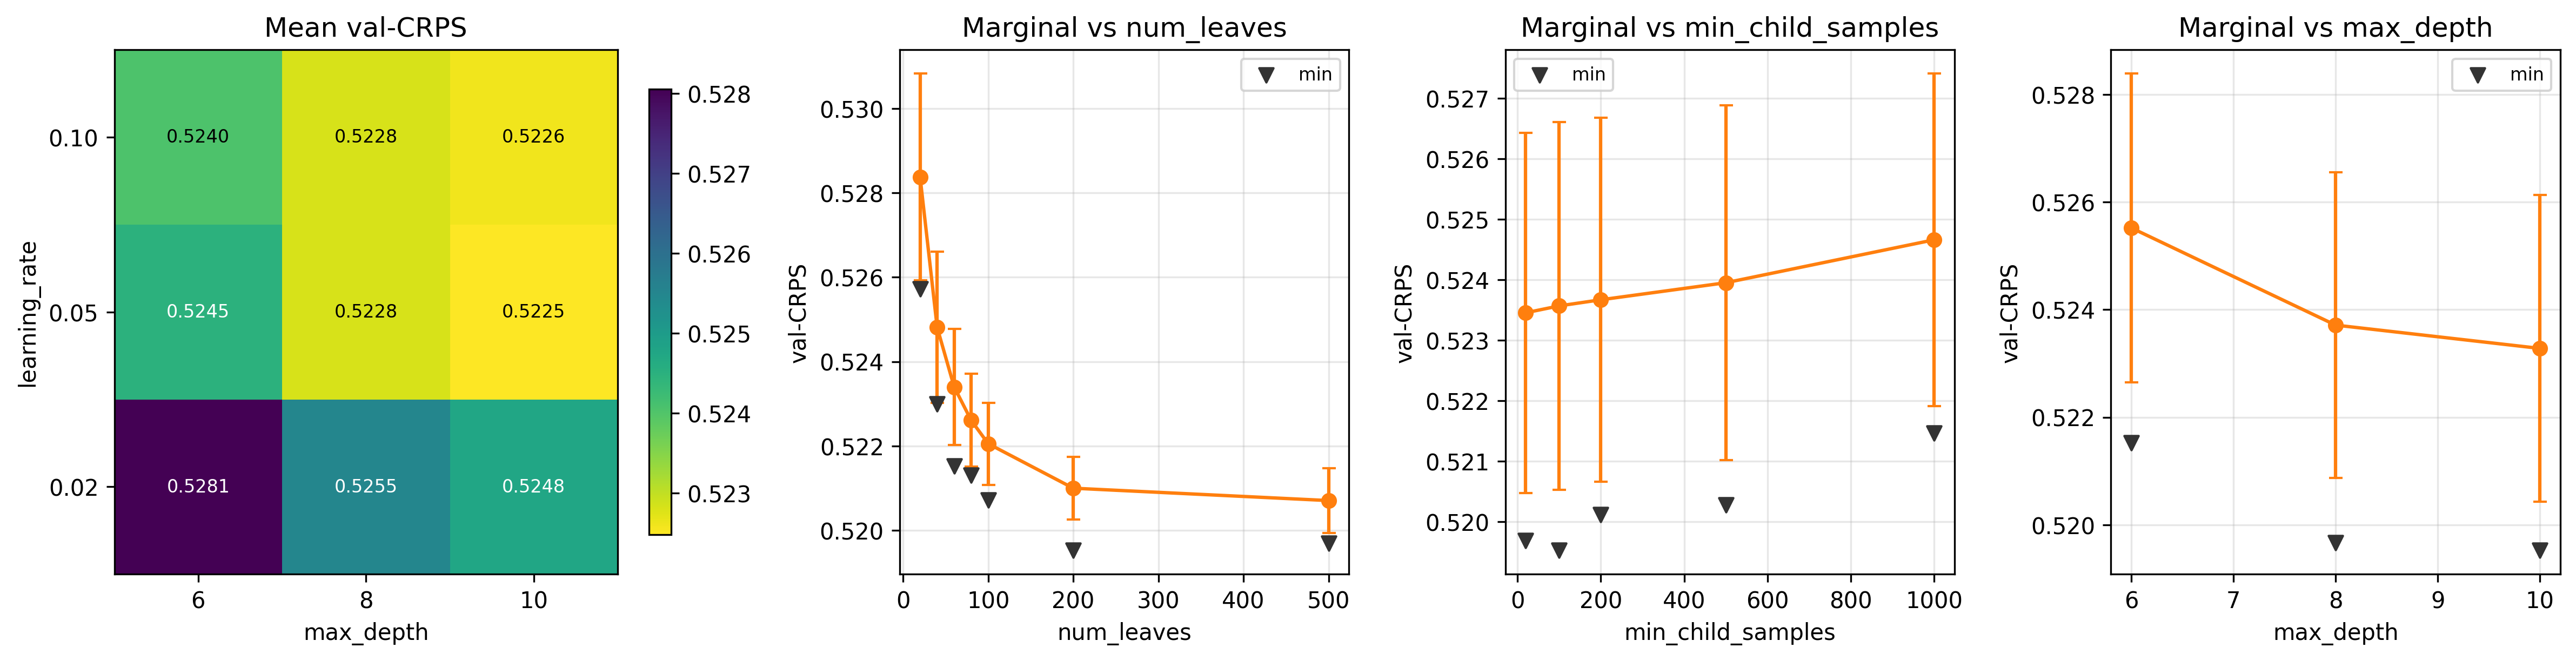
\includegraphics[width=0.99\textwidth]{images/05/lgbm_hpo}
    \caption{Hyperparameter optimisation over the 240-combination
    grid. Left: mean fold-averaged CRPS as a function of
    \texttt{max\_depth} and \texttt{learning\_rate}. Right: marginal
    fold-averaged CRPS along the \texttt{num\_leaves},
    \texttt{min\_child\_samples} and \texttt{max\_depth} axes; the
    orange curves show the per-axis mean with $\pm 1\sigma$ error
    bars and the black markers indicate the per-axis minimum}
    \label{fig:lgbm-hpo}
\end{figure}

\clearpage

%=============================================================================
\section{Cross-validation results}
\label{sec:lgbm-cv-results}
%=============================================================================

\subsection{Per-fold CRPS and MAE}
\label{sec:lgbm-perfold}

Table~\ref{tab:lgbm-cv} reports the per-fold CRPS and MAE for the
five-fold cross-validation. The standard deviation across folds is
small (${\approx}1{.}6\,\%$ of the mean for CRPS) and consistent
with the homogeneous spatial coverage of the fold partition.

\begin{table}[ht]
  \centering
  \caption{5-fold cross-validation results for LightGBM. Each row
  reports the CRPS and MAE on the held-out fold, computed in
  physical millimetres on the predicted-wet records. The last row
  reports the mean across folds with the corresponding standard
  deviation}
  \label{tab:lgbm-cv}
  \begin{tabular}{c r r r}
    \toprule
    Fold & $n_{\mathrm{test}}$ & MAE (mm) & CRPS (mm) \\
    \midrule
    0 & 3{,}520{,}827 & 1.066 & 0.804 \\
    1 & 3{,}466{,}145 & 1.056 & 0.796 \\
    2 & 3{,}495{,}450 & 1.040 & 0.787 \\
    3 & 3{,}471{,}152 & 1.023 & 0.774 \\
    4 & 3{,}452{,}880 & 1.024 & 0.777 \\
    \midrule
    \textbf{Mean} & --- & $\mathbf{1.042 \pm 0.019}$
                       & $\mathbf{0.788 \pm 0.013}$ \\
    \bottomrule
  \end{tabular}
\end{table}


\subsection{Error stratification}
\label{sec:lgbm-errors}

Figure~\ref{fig:lgbm-crps-intensity} stratifies the OOF CRPS by
true precipitation intensity. Light to moderate rainfall events
(0.5--10~mm) dominate the record and are predicted with
sub-millimetre CRPS. Skill degrades approximately linearly on the
upper tail: the heaviest bin ($\geq 50$~mm) reaches CRPS values an
order of magnitude larger than the body.
Figure~\ref{fig:lgbm-spatial-errors} maps the per-station OOF MAE
across the study area; errors are spatially smooth and concentrated
along the elevated south-eastern corner of the domain, mirroring
the pattern observed in the kriging cross-validation
(Section~\ref{sec:kriging-evaluation}).

\begin{figure}[H]
    \centering
    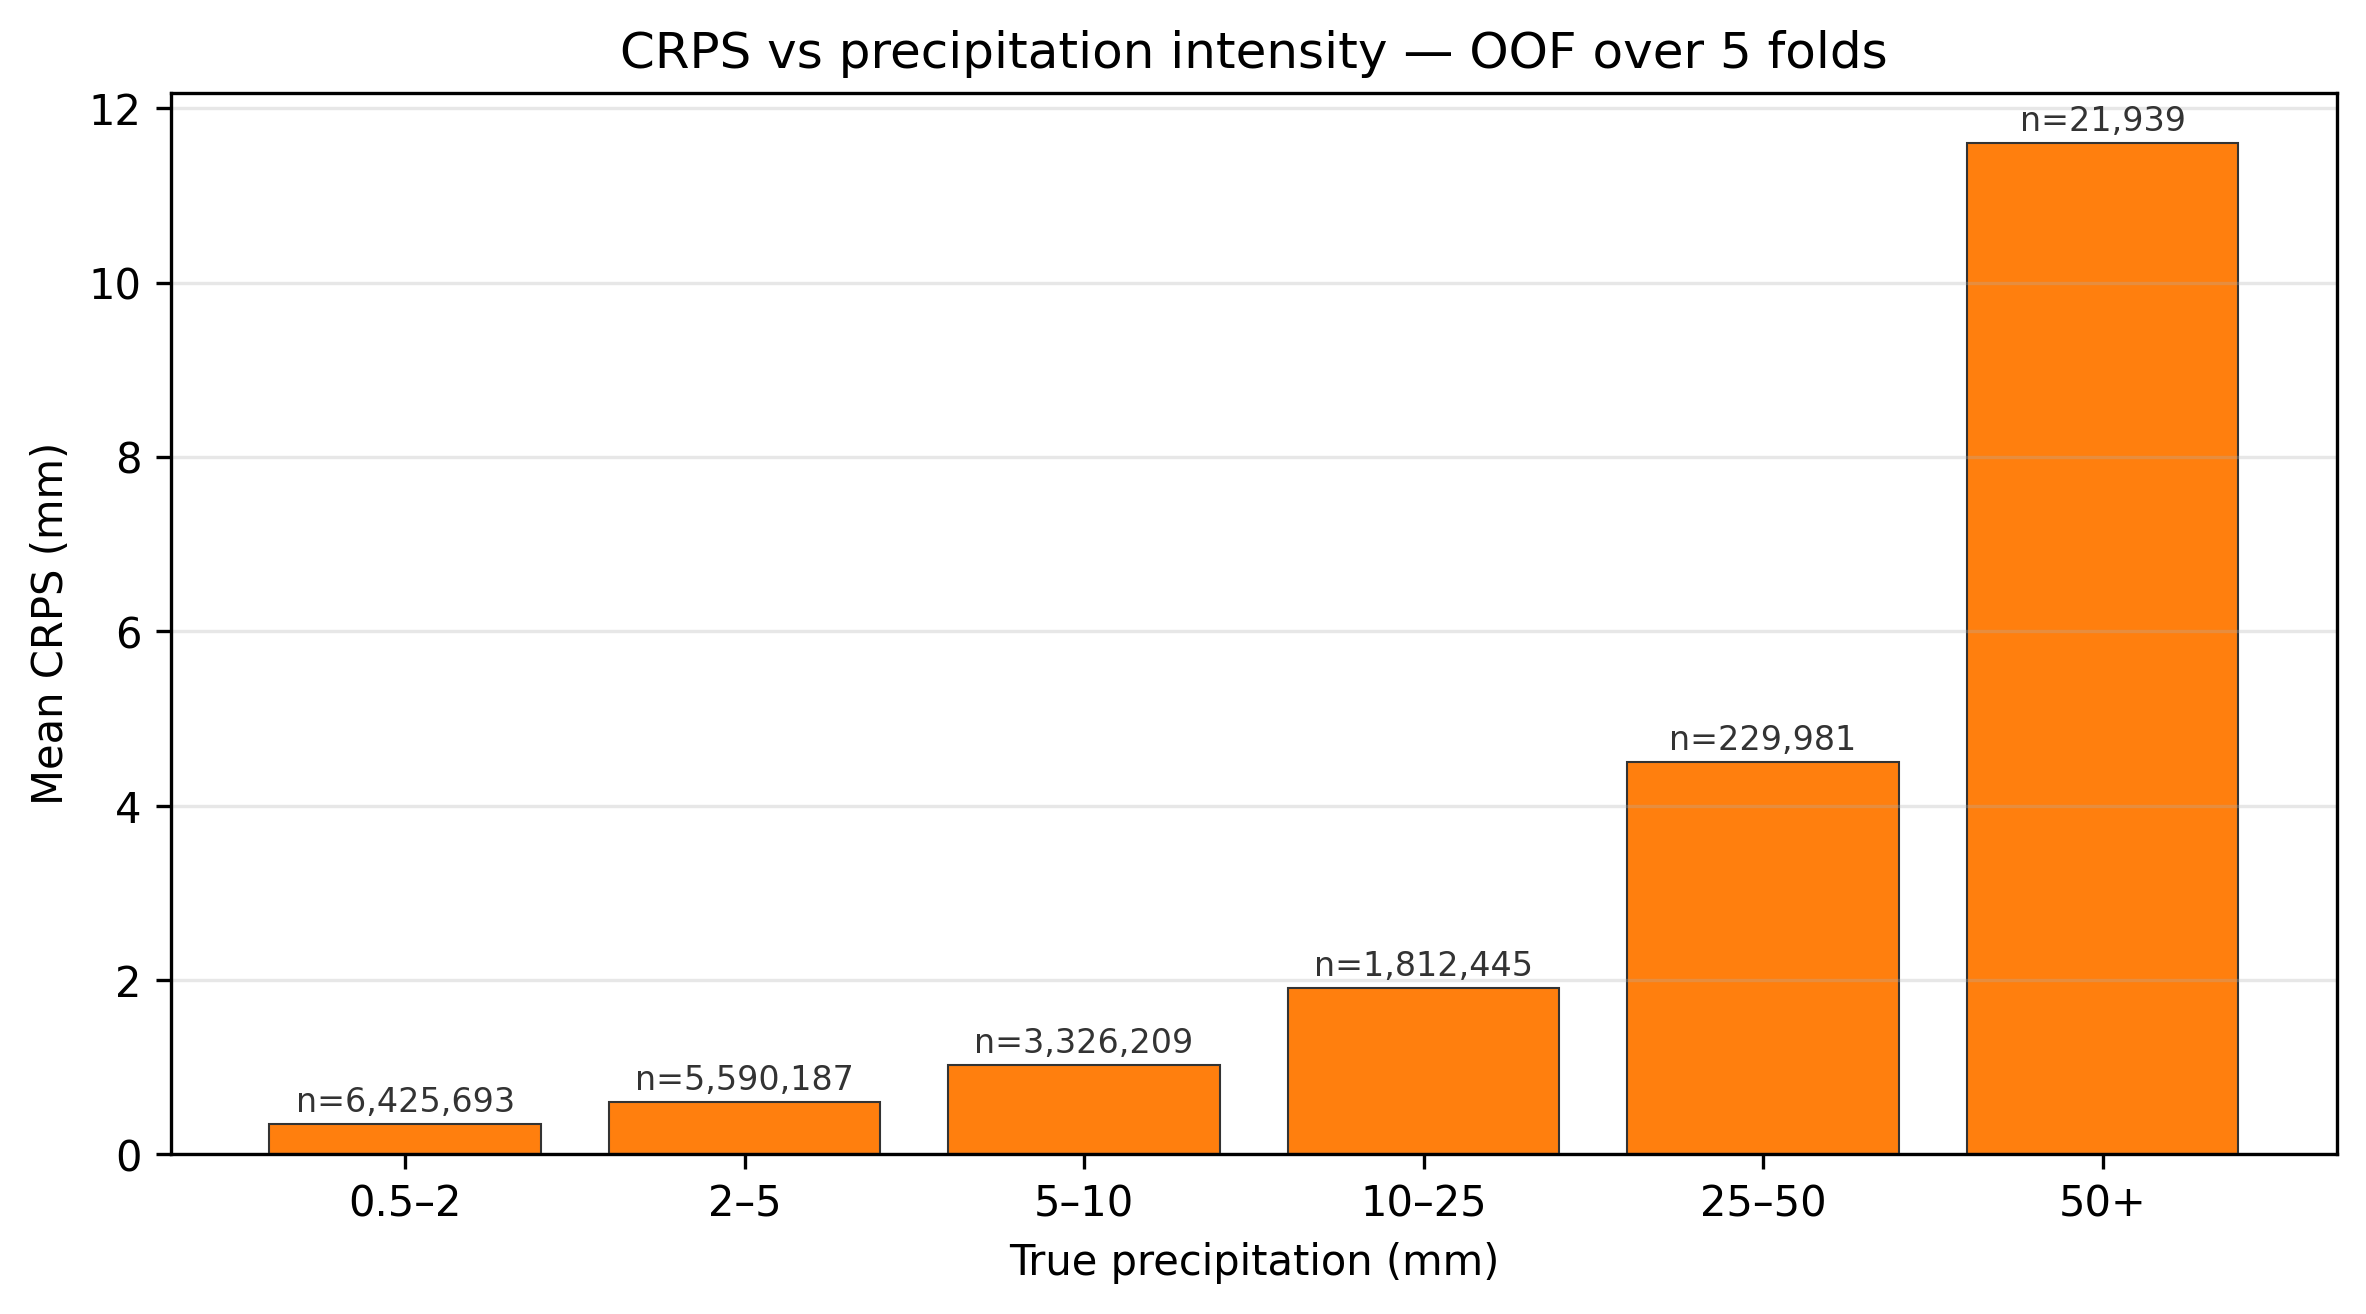
\includegraphics[width=0.85\textwidth]{images/05/lgbm_crps_by_intensity}
    \caption{Out-of-fold CRPS stratified by true precipitation
    intensity. Bars annotated with the bin sample size $n$}
    \label{fig:lgbm-crps-intensity}
\end{figure}

\begin{figure}[H]
    \centering
    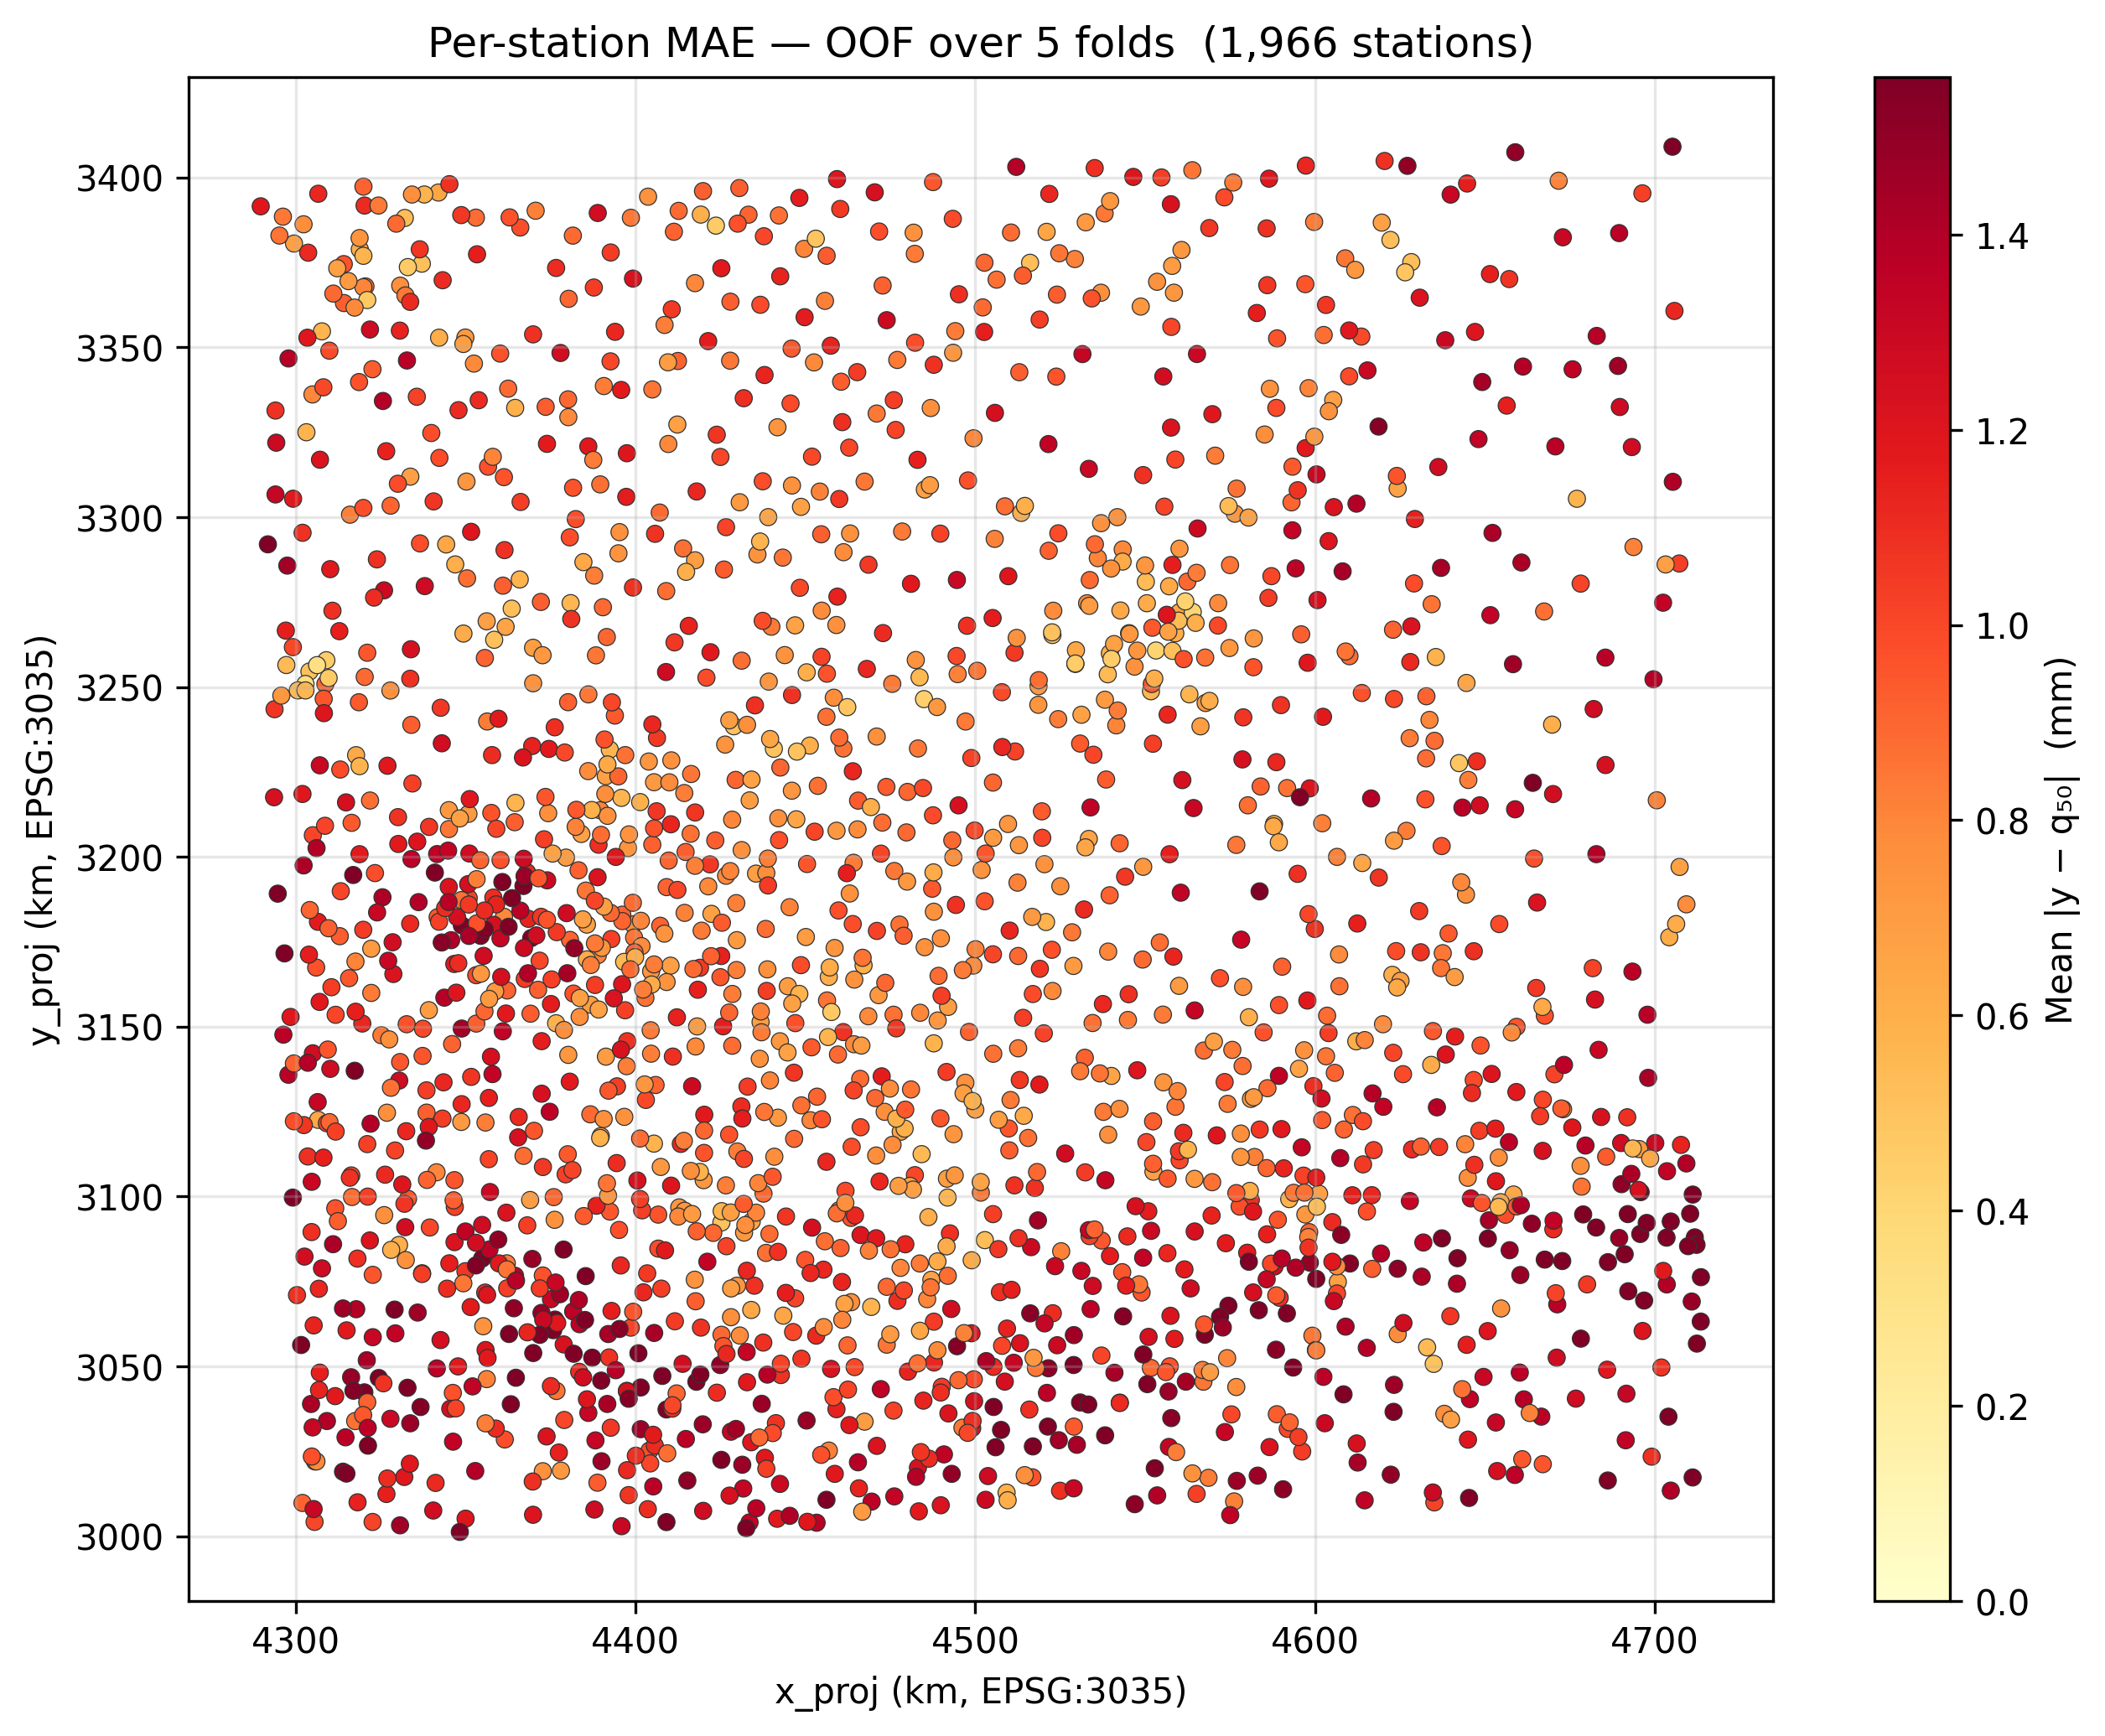
\includegraphics[width=0.85\textwidth]{images/05/lgbm_spatial_errors}
    \caption{Per-station out-of-fold MAE across the study area.
    Each station appears in exactly one fold's test side, so the
    colour at a point is the OOF mean residual at that location}
    \label{fig:lgbm-spatial-errors}
\end{figure}
\clearpage

%=============================================================================
\section{Discussion}
\label{sec:lgbm-discussion}
%=============================================================================

\subsection{Feature importance}
\label{sec:lgbm-feature-importance}

\begin{figure}[H]
    \centering
    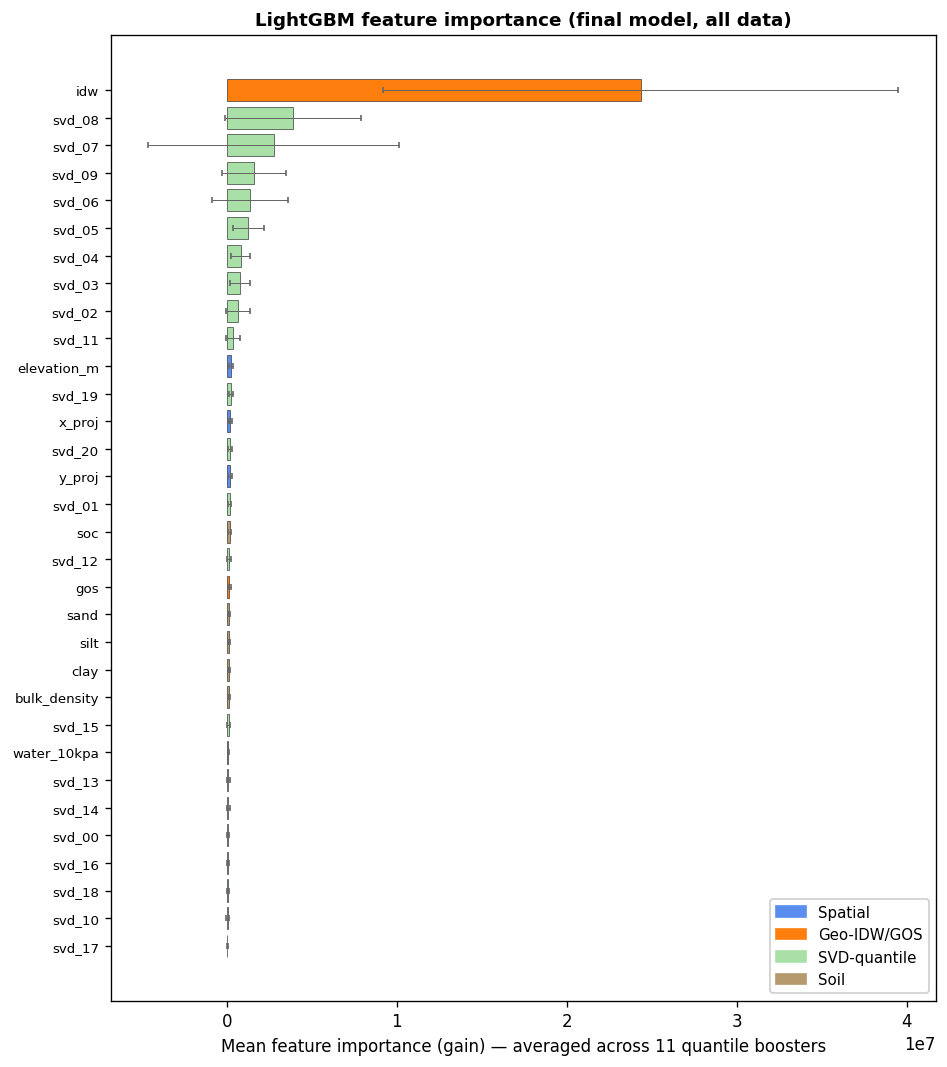
\includegraphics[width=0.48\textwidth]{images/05/features_importants_gain}\hfill
    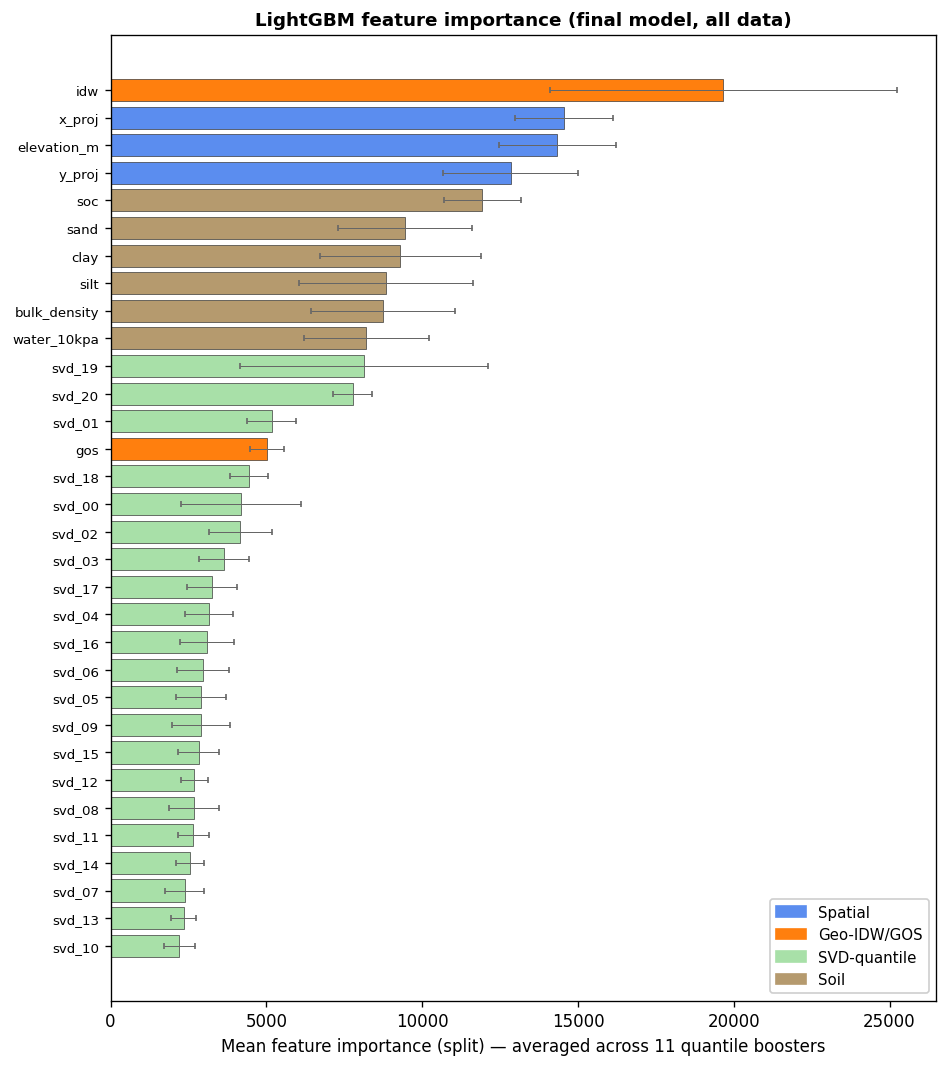
\includegraphics[width=0.48\textwidth]{images/05/features_importants_split}
    \caption{LightGBM feature importance averaged across the eleven
    quantile boosters of the final model, ranked by two complementary
    metrics. Left: \emph{gain} importance, the total reduction in
    pinball loss attributed to each feature across all splits. Right:
    \emph{split count}, the number of times each feature is used as a
    split variable. Bars are colour-coded by feature group; error bars
    indicate the cross-quantile standard deviation}
    \label{fig:lgbm-features}
\end{figure}

Figure~\ref{fig:lgbm-features} reports the per-feature importance under
both LightGBM metrics. The two views tell complementary stories.

By \emph{gain}, the inverse-distance-weighted mean \texttt{idw} dominates
by a wide margin, followed by a second tier of central SVD-quantiles
(\texttt{svd\_07}--\texttt{svd\_09}). A single split on \texttt{idw}
captures most of the spatial signal in the target, because the average of
the $K=15$ nearest wet-day neighbours is by itself a strong predictor of
the local precipitation amount. The central SVD-quantiles refine that
prediction on heterogeneous neighbourhoods where the mean alone
under-describes the rainfall pattern.

By \emph{split count}, the static spatial coordinates
($x_{\mathrm{proj}}$, $y_{\mathrm{proj}}$, \texttt{elevation\_m}) and the
SoilGrids covariates contribute substantially: each receives many splits
even though every individual split contributes little to the loss
reduction. This is the typical signature of \emph{local fine-tuning
features}: once the dominant \texttt{idw}/SVD signal has been captured by
a few high-gain splits, the trees use the static covariates repeatedly to
correct the residuals in narrow regions of the feature space. The two
metrics therefore agree on the hierarchy of the dynamic FFRK features as
the principal signal carriers, while showing that the static spatial and
soil covariates are not redundant: they are used frequently, but for a
different purpose.

\subsection{Why no residual kriging}
\label{sec:lgbm-rk-ablation}

The choice of direct quantile regression over a regression-kriging
hybrid (LightGBM trend plus Ordinary Kriging on residuals) was
guided by a dedicated ablation on the same 5-fold partition used for
the main model (Section~\ref{sec:lgbm-training}). The dynamic
neighbourhood feature set (IDW, SVD-quantiles, geographically
oriented statistics) already absorbs the spatial signal, so the
residual field is near-white-noise spatially: the fitted residual
variogram exhibits a pure-nugget structure with negligible
psill-to-sill ratio. Kriging an essentially uncorrelated residual
field adds variance without reducing bias, and the hybrid model
underperformed direct quantile regression on holdout CRPS in every
fold. Direct quantile regression is therefore preferred: fewer
moving parts and a closed-form CRPS via the eleven-member ensemble,
with no parametric back-transformation step.
